% =================================================================================================
% File:			processi_organizzativi.tex
% Description:	Definisce il capitolo deei processi organizzativi
% Created:		2014/12/11
% Author:		Tesser paolo
% Email:		tesser.paolo@mashup-unipd.it
% =================================================================================================
% Modification History:
% Version		Modifier Date		Change												Author
% 0.0.1 		2014/12/11 			Inizializzazione del file							Tesser Paolo
% =================================================================================================
% 0.0.2			2014/12/12			Inizio stesura della struttura dei sottocapitoli	Tesser Paolo
% =================================================================================================
% 0.0.3			2014/12/14			Inizio stesura sottosezione processi di gestione	Tesser Paolo
% =================================================================================================
% 0.0.4			2014/12/16			Miglioramento sottosezioni e continuata stesura		Tesser Paolo
% =================================================================================================
% 0.0.5			2014/12/20			Inseriti ruoli di progetto e alcuni strumenti		Tesser Paolo
% =================================================================================================
% 0.0.6			2014/12/23			inseriti diagrammi su alcune procedure				Tesser Paolo
% =================================================================================================
% 0.0.7			2014/12/26			completate procedure e diagrammi in gestione proc	Tesser Paolo
% =================================================================================================
%

% CONTENUTO DEL CAPITOLO

\section{Processi Organizzativi}

	\subsection{Gestione dei Processi}
		\subsubsection{Attività}
			\paragraph{Gestione delle Comunicazioni}
					\subparagraph{Mail}
					\label{sec:mail}
					Ogni membro del gruppo avrà una mail personale creata grazie all'acquisizione di un dominio web sul servizio di hosting NetSons. \\
					Il formato dell'indirizzo dovrà essere del tipo esposto di seguito e servirà per registrarsi ad ogni servizio che il team andrà ad utilizzare:
						\begin{center}
							cognome.nome@mashup-unipd.it
						\end{center}
												
				\subparagraph{Comunicazioni interne}
				\label{sec:comunicazioni_interne}
				Le comunicazione interne e prettamente informali verranno gestite tramite un gruppo su WhatsApp denominato MashUp. \\
				Quelle formali avverranno attraverso il sistema di ticketing Asana che consente una chat di gruppo al suo interno e che notifica a tutti gli altri membri tramite mail quando qualcuno scrive qualcosa in essa. \\
				Le norme e le procedure relative a questo servizio verranno trattate in dettaglio nella sezione \ref{sec:gestione_dei_task} e in quella \ref{sec:asana}. \\
				Se si necessita di un interazione vocale con gli altri membri, qualora non fossero presenti nello stesso luogo, verrà utilizzata l'applicazione Skype.
				\subparagraph{Comunicazioni esterne}
				\label{sec:comunicazioni_esterne}
				Le comunicazione esterne vengono effettuate dal \roleProjectManager{} in quanto rappresenta il gruppo \groupName. \\
				Egli, attraverso la seguente mail, manterrà i contatti con il proponente e con il committente. In caso lo ritenga necessario, girerà tali messaggi agli altri membri del team.
					\begin{center}
						info@mashup-unipd.it
					\end{center}
					\'E stato inoltre stabilito, insieme al proponente, che l'interazione con lui, qualora non potesse avvenire tramite un incontro esterno, specificato nella sezione \ref{sec:riunioni_esterne}, possa avvenire tramite videochiamata in Skype	e condividendo parte dei documenti del progetto.	
			\paragraph{Gestione delle Riunioni}
				\subparagraph{Riunioni interne}
				Il \roleProjectManager{} ha il compito di convocare le riunioni interne al team. Dovrà quindi informare i componenti tramite le metodologie viste nella sezione \ref{sec:comunicazioni_interne}.\\
				Per ogni nuovo incontro dovranno essere specificati la data, l’ora, il luogo, il proponente e la motivazione che lo hanno reso necessario. \\
				Ad ogni membro del gruppo è consentito chiedere la convocazione di una riunione interna. Il \roleProjectManager{}, una volta valutati i motivi e la necessità di tale incontro, provvederà ad organizzarlo secondo le norme viste in precedenza.
				\subparagraph{Riunioni esterne} \label{sec:riunioni_esterne}
				Il \roleProjectManager{} ha il compito di concordare la data, l’ora e il luogo dell'incontro con il proponente o con il committente attraverso 	il meccanismo visto nella sezione \ref{sec:comunicazioni_esterne}. \\
				Una volta trovato l'accordo dovrà notificarlo agli altri membri secondo i metodi presenti nella sezione \ref{sec:comunicazioni_interne}. \\
				Ad ogni membro del gruppo è consentito chiedere la convocazione di una riunione esterna. Il \roleProjectManager, oltre ad accertarsi dei motivi e delle necessità di tale incontro, dovrà garantire che siano presenti almeno due componenti del team. Sarà compito di uno dei presenti, delegato di volta in volta, redigere il verbale dell’incontro avvenuto.
				
			\paragraph{Gestione dei task}
			\label{sec:gestione_dei_task}
			Il \roleProjectManager{} deve pianificare e assegnare i compiti che i singoli membri dovranno andare a eseguire. Per farlo viene usato l'applicazione web Asana che consente di creare facilmente i task. \\
			Permette inoltre un buon monitoraggio dell'andamento globale del progetto, offrendo grafici che illustrano il rapporto tra i ticket completati e quelli ancora da terminare in relazione anche alle milestone fissate dal team.
			
			\paragraph{Gestione dello svolgimento dei task} % (fold)
			\label{par:gestione_dello_svolgimento_dei_task}
			Ogni membro del team è tenuto ad accettare tutti i task che il \roleProjectManager{} pianificherà di assegnarli. \\
			Se per dei motivi eccezionali l'assegnatario non potesse svolgere il compito indicato dovrà renderlo noto nei modi previsti nella sezione \ref{sec:comunicazioni_interne} al \roleProjectManager, il quale, una volta valutate le motivazione, dovrà provvedere a trovare un nuovo destinatario del task. \\
			Qualora il \roleProjectManager{} non ricevesse alcuna notifica entro le prime 24 ore riterrà automaticamente accettato il task dall'assegnatario.
			% paragraph gestione_dello_svolgimento_dei_task (end)
			
			\paragraph{Gestione delle change request}
			(NOTA: DA SPOSTARE NEL PROCESSO DI SUPPORTO -> Risoluzione di Problemi) \\
			Ogni membro del team può proporre dei cambiamenti o degli avanzamenti da apportare. Il suggerimento dovrà essere motivato adeguatamente in modo che il \roleProjectManager{} non debba preoccuparsi di ricercare le fonti che forniscono l'effettiva validità di questo mutamento. \\
			Una volta verificata o meno la necessità dell'idea, il \roleProjectManager{} approverà o respingerà la proposta fatta. \\
			Qualora la proposta fosse accettata il \roleProjectManager{} avrà il compito di pianificare le attività che serviranno ad apportare il cambiamento.
			
			\paragraph{Gestione della commit}
			Per fornire al \roleProjectManager{} un più ampio quadro di come stanno procedendo i singoli compiti viene utilizzato un servizio web offerto da GitHub. \\
			Questo permette di mostrare nei commenti dei task il messaggio inserito durante la commit una volta effettuata l'operazione di push sul server. \\
			Fornisce quindi il tracciamento del lavoro che viene svolto per portare a compimento il task in questione.
			Il servizio viene attivato sia in doc\_BDSM\_App sia in src\_BDSM\_App.
				\subparagraph{Meccanismo di aggancio commit-task} % (fold)
				\label{subp:meccanismo_di_aggancio_commit_task}
				\'E stato creato un account generale su Asana con user name ``MainMashUp'' che fornisce l'API\_Key necessaria a configurare il servizio senza che esso dipenda dall'account di un membro in particolare. \\
				Per permettere il tracciamento bisogna usare l'identificato del task di cui vogliamo tracciare i messaggi di commit.\\
				L'id si può reperire nel modalità illustrate dalla figura \ref{fig:select_id_task_asana} e va inserito all'interno del messaggio nelle modalità indicate nella sezione \ref{sec:messaggio_di_commit}
					
				% subparagraph meccanismo_di_aggancio_commit_task (end)

			
		\subsubsection{Procedure}
			\paragraph{Procedura d'assegnazione dei task}
			\label{par:procedura_assegnazione_task}
			Il \roleProjectManager{} dovrà eseguire i seguenti passi, riassunti in seguito nella figura \ref{fig:procedura_assegnazione_task}. \\
			Per effettuare più velocemente un'assegnazione si potrà servire del template illustrato nella figura \ref{fig:template_task_asana}.
				\begin{enumerate}
					\item definire il titolo del task secondo le norme presenti nella sezione \ref{par:formato_dei_task};
					\item se necessario, fornire una descrizione più esaustiva del compito da svolgere;
					\item definire la data di scadenza entro la quale il task dovrà essere portato a termine;
					\item indicare il verificatore;
					\item aggiungere tra i followers del task l'utente: ``MainMashUp'';
					\item selezionare l'assegnatario del task. Questa assegnazione genererà in automatico una notifica al membro scelto;
					\item se si dovesse verificare il caso in cui l'assegnatario rifiutasse il task assegnato e il \roleProjectManager{} accertasse questa impossibilità nel suo svolgimento, dovrà eseguire di nuovo il passo precedente. 
				\end{enumerate}
				\begin{figure}
					\centering
					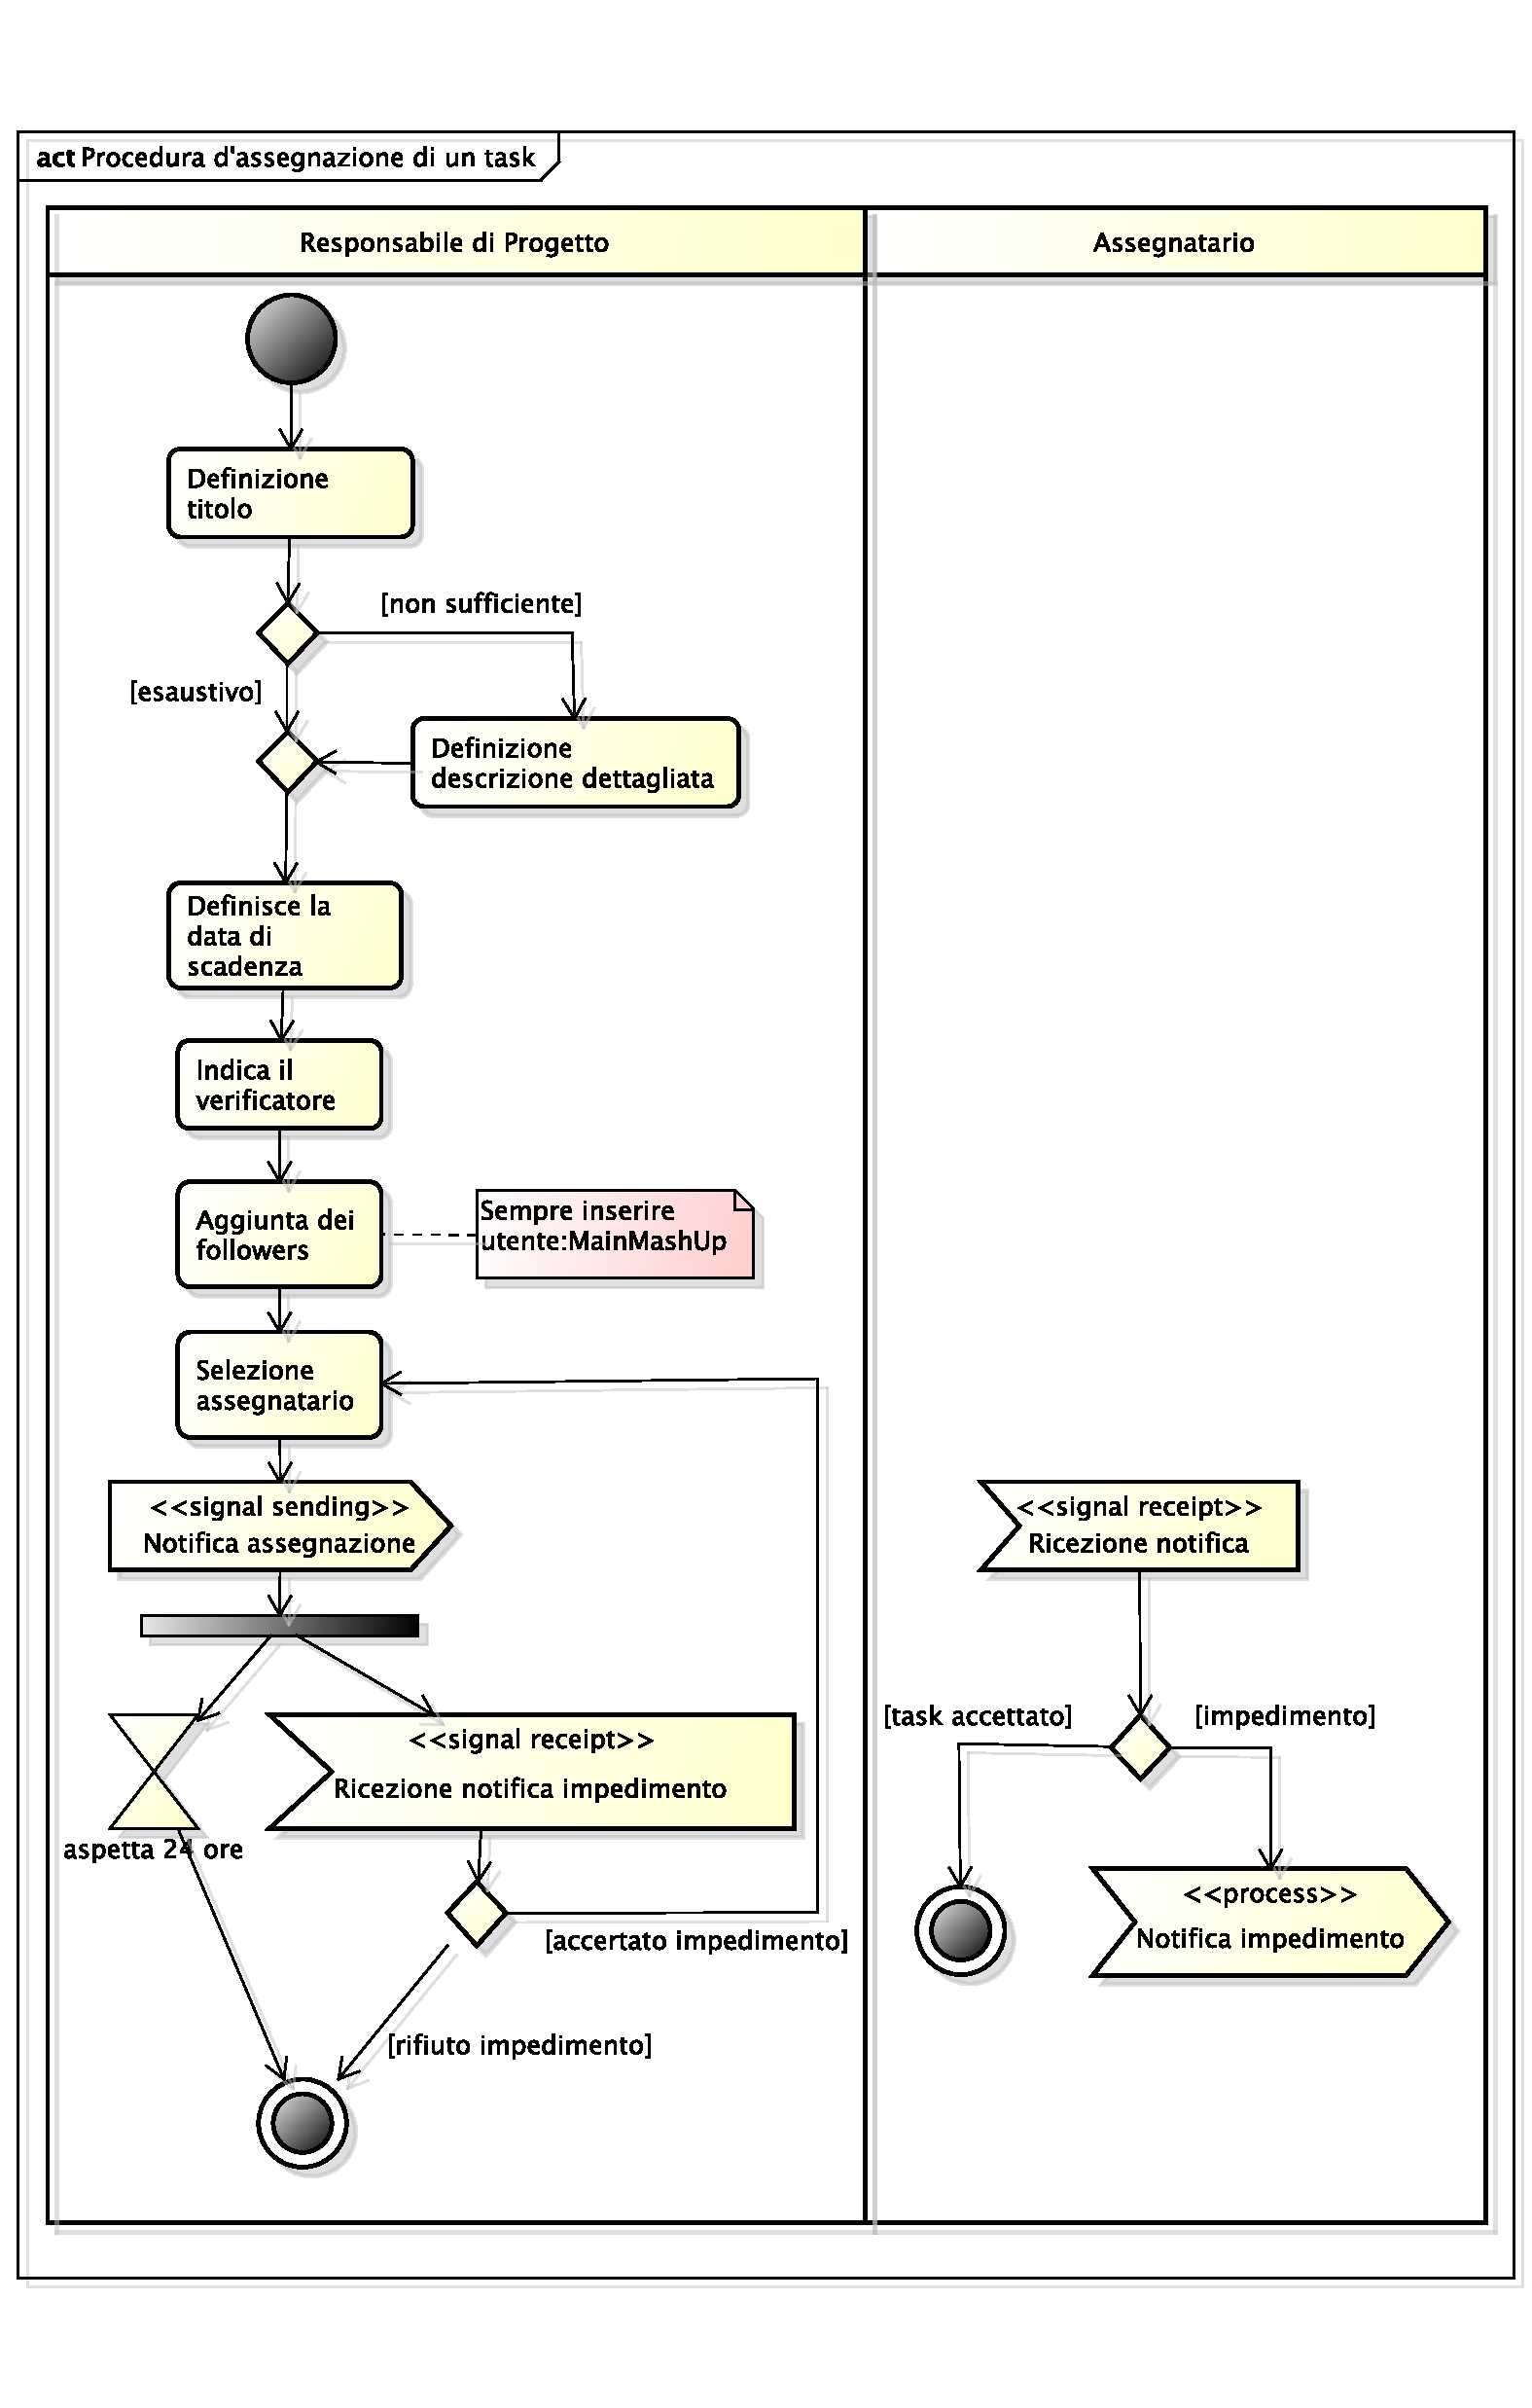
\includegraphics[width=14cm]{images/proc_assegnazione_task.pdf}
					\caption{Diagramma di attività - procedura d'assegnazione di un task}
					\label{fig:procedura_assegnazione_task}
				\end{figure}
				
			\paragraph{Procedura per il reperimento dell'id del task}
			\label{par:procedura_reperimento_id_task_asana}
			Ogni membro che vorrà recuperare l'identificativo del task su cui sta lavorando dovrà:
				\begin{enumerate}
					\item entrare su Asana;
					\item posizionarsi sul task che si sta lavorando dalla sezione ``MyTasks'';
					\item posizionarsi sull'url e copiare tutte le cifre dopo l'ultimo slash ``/''. Quello è l'id che si sta cercando.
				\end{enumerate}
				
				\begin{figure}[htbp]
					\centering
					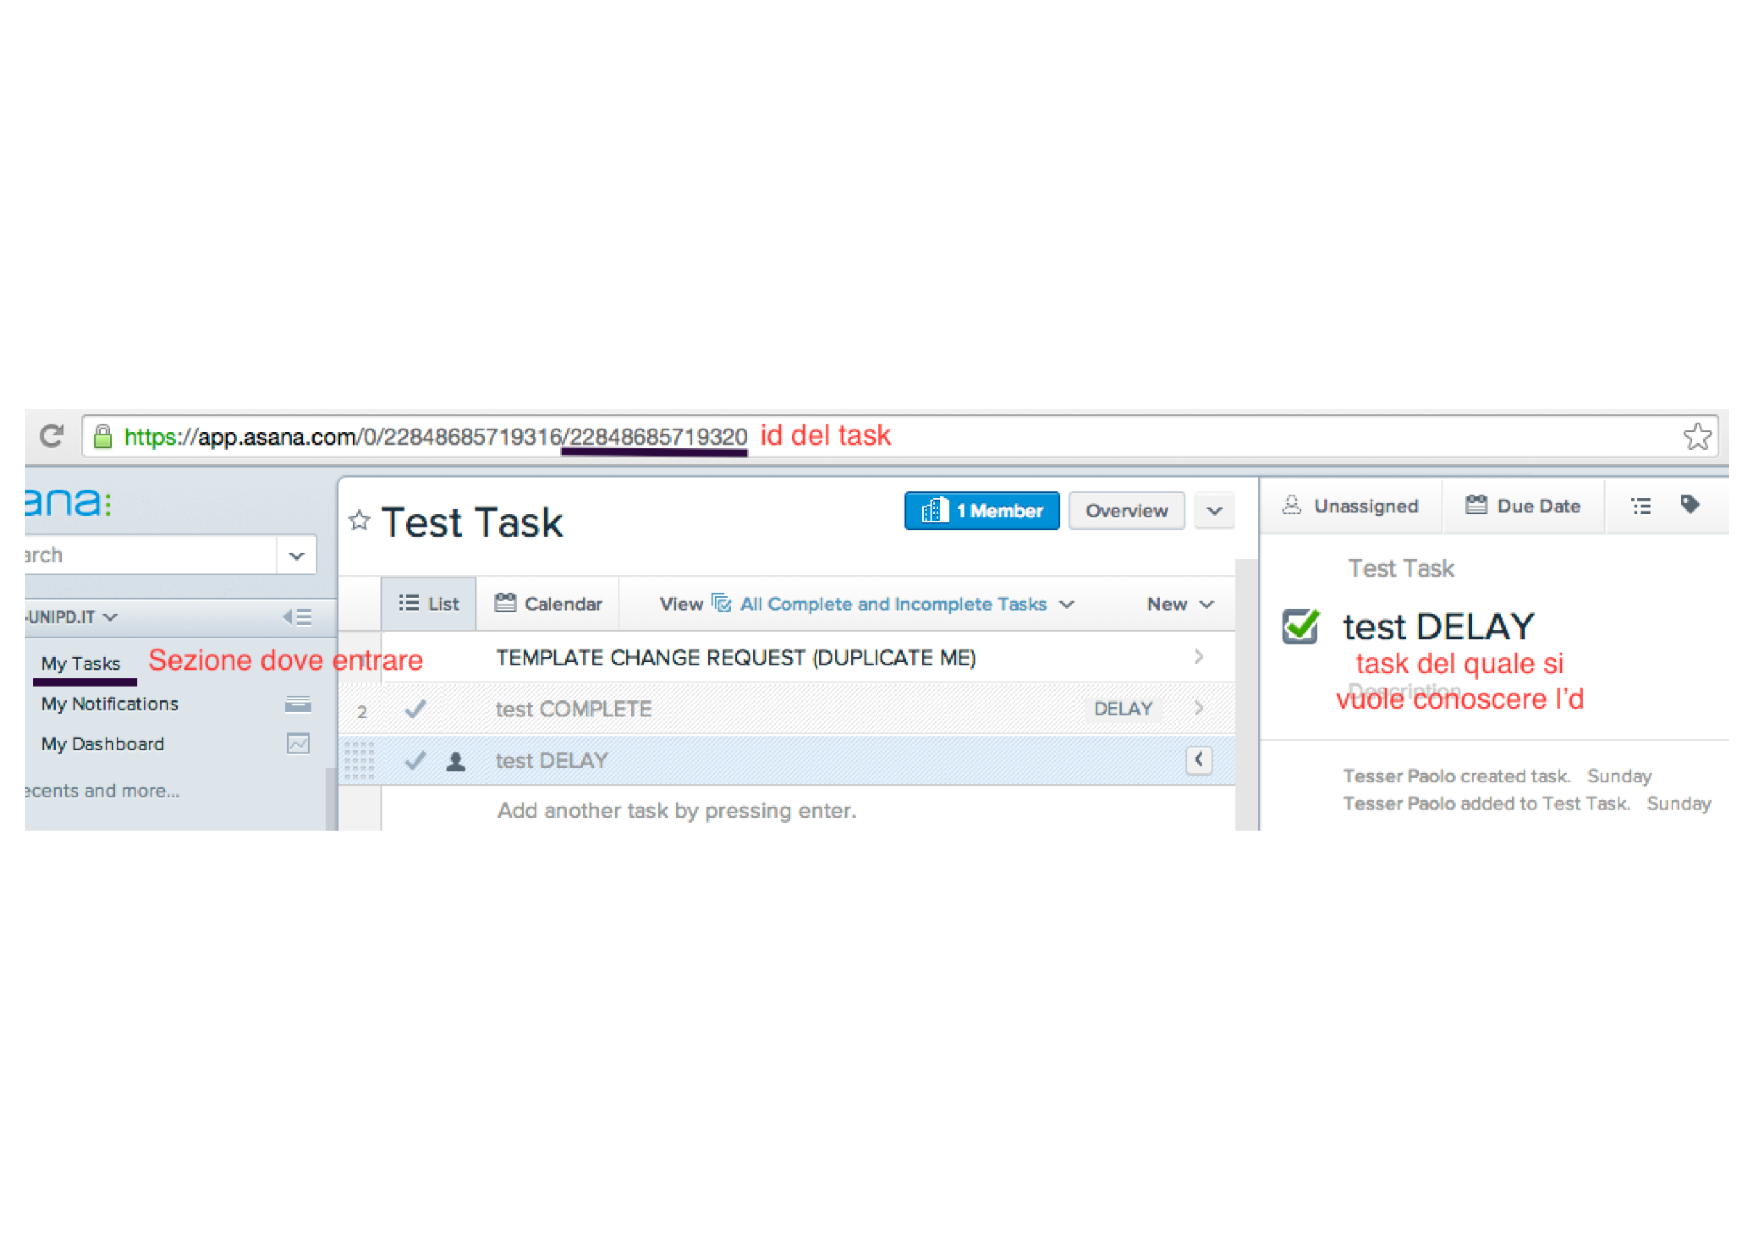
\includegraphics[width=14cm]{images/select_id_task_asana.pdf}
					\caption{Reperimento dell'id del task}
					\label{fig:select_id_task_asana}				
				\end{figure}
			
			\paragraph{Procedura di svolgimento dei task assegnati}
			Il membro assegnatario del task, una volta ricevuta la notifica e non avendo nessuna motivazione per rifiutarlo, dovrà:
				\begin{enumerate}
					\item se il task ha una scadenza più immediata rispetto a quella del task sui cui si sta lavorando, sospendere lo svolgimento del task con data di scadenza più lontana e procedere con quello appena notificato, altrimenti metterlo in coda;
					\item se dopo avere iniziato l'esecuzione del task, si riceve la notifica di uno nuovo con scadenza più immediata, si dovranno sospendere le attività che portano al compimento del task con scadenza meno ravvicinata ed eseguire nuovamente il passo precedente;
					\item se per svolgere il compito si dovesse andare oltre la data di scadenza prevista, si deve impostare il tag ``DELAY'' dal sistema Asana o tramite i modi espressi nella sezione \ref{sec:messaggio_di_commit}. \\
					Questa situazione si può verificare se:
					 	\begin{itemize}
							\item il tempo assegnato dal \roleProjectManager{} è inferiore a quanto richiesto per il compimento del task;
							\item il task può essere completato solo quando un altro task sia portato a termine. Queste dipendenze devono verificarsi il meno possibile ed è compito del \roleProjectManager{} evitare ciò in fase di pianificazione;
					 		\item l'assegnatario ha rallentamenti esterni non resi noti al \roleProjectManager{} in fase di pianificazione;
							\item il compimento del task necessità di competenze non in possesso dell'assegnatario.
					 	\end{itemize}
					\noindent
					Nei primi due casi la responsabilità è imputabile al \roleProjectManager, mentre negli ultimi due la responsabilità è del membro che devo svolgere il task;
					\item al completamento del task, dovrà chiudere il task, spuntandolo direttamente dal sistema Asana o tramite i modi espressi nella sezione \ref{sec:messaggio_di_commit};
					\item l'operazione illustrata al passo precedente genera in automatico una notifica verso il \roleVerifier{} e il \roleProjectManager;
					\item ritornare al primo punto con i task rimanenti. 

				\end{enumerate}
				
				\begin{figure}[htbp]
					\centering
					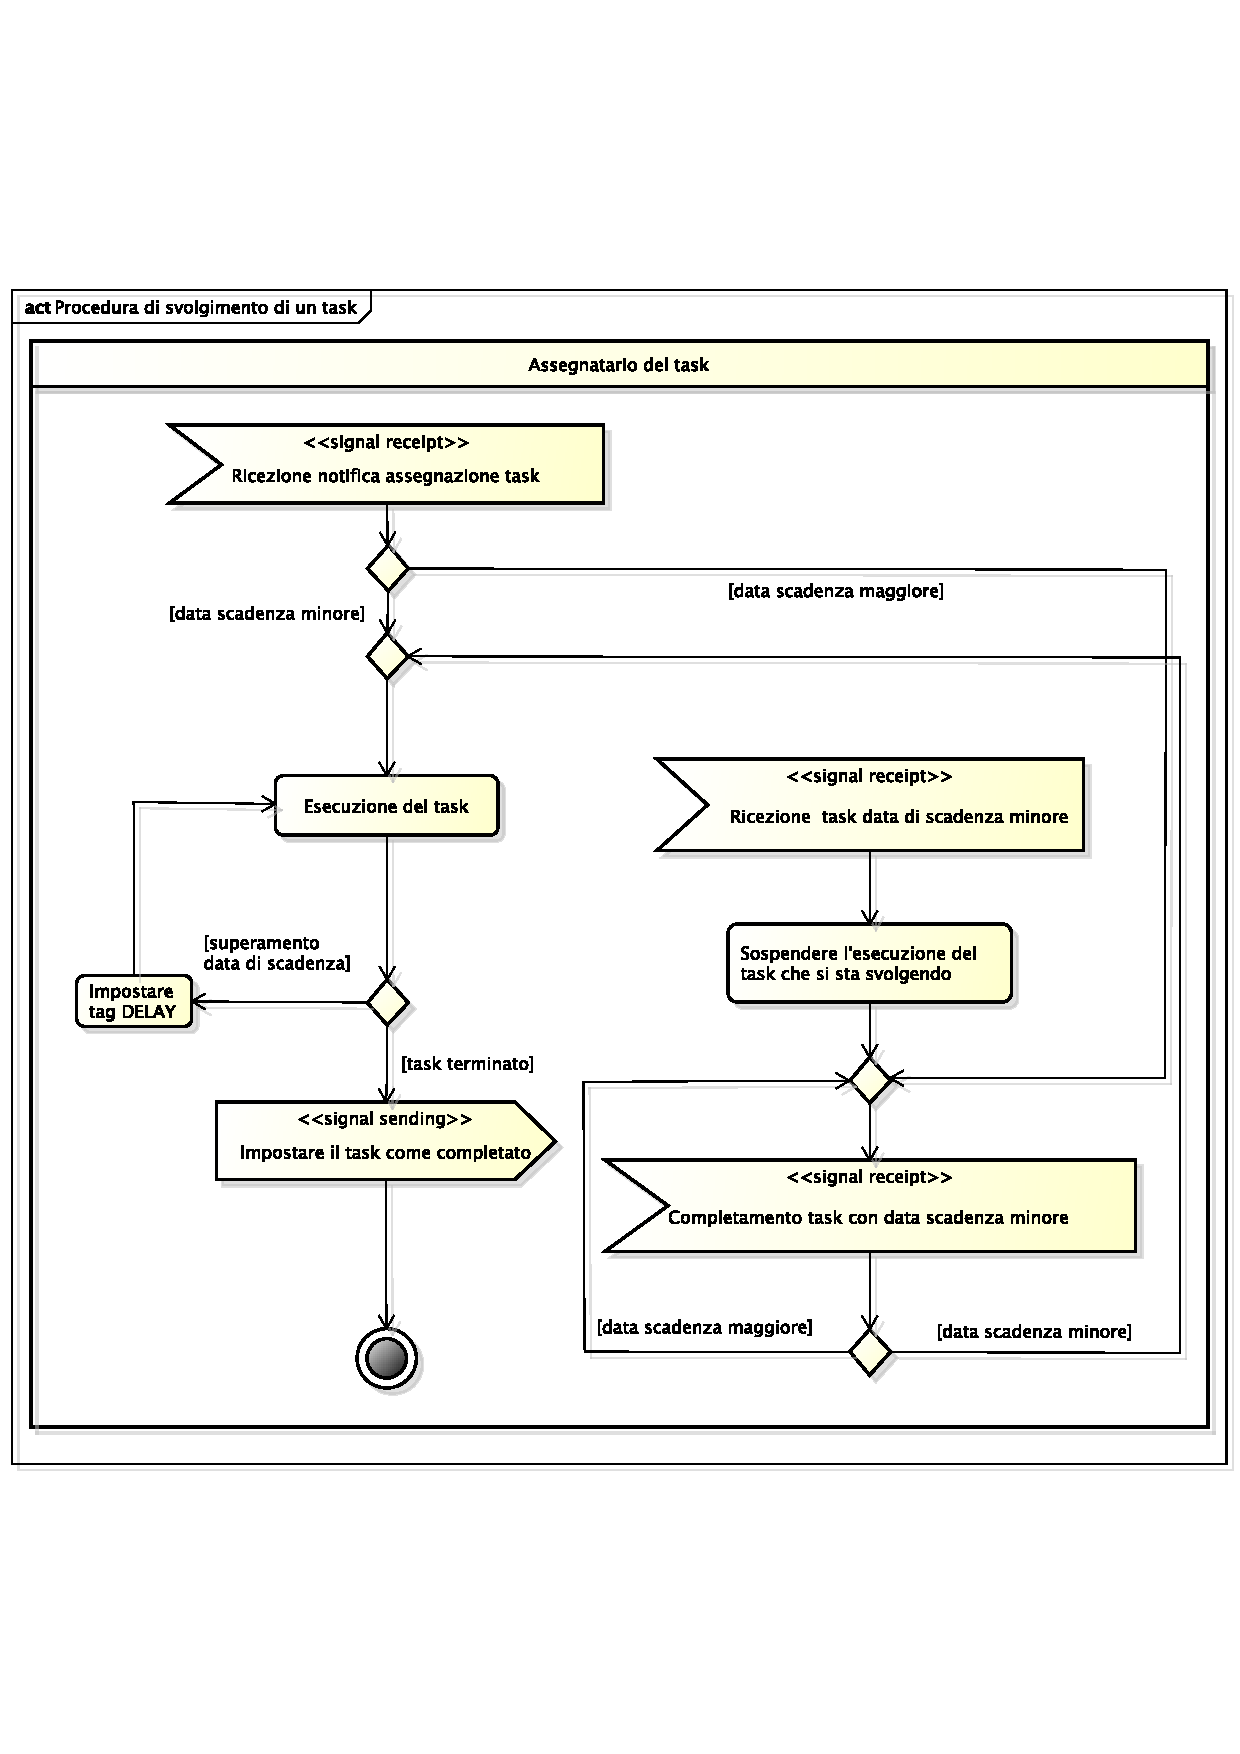
\includegraphics[width=14cm]{images/proc_svolgimento_task.pdf}
					\caption{Diagramma di attività - procedura di svolgimento dei task assegnati}
					\label{fig:procedura_svolgimento_task}				
				\end{figure}
				
			\paragraph{Procedura di svolgimento di una change request}
			(NOTA: DA SPOSTARE NEL PROCESSO DI SUPPORTO -> Risoluzione di Problemi) \\
			Ogni membro del gruppo, che intenda proporre dei cambiamenti o introdurre degli avanzamenti, è tenuto a seguire questa procedura . \\
			Per effettuare più velocemente l'apertura di una change request si potrà servire del template illustrato nella figura \ref{fig:template_change_request_asana}.
				\begin{enumerate}
					\item definire il titolo del cambiamento/avanzamento;
					\item definire una descrizione dettagliata del motivo che ha portato alla proposta e le fonti che garantiscono la bontà del cambiamento/avanzamento che si vuole attuare;
					\item selezionare il \roleProjectManager{} in carica. Questa assegnazione genera in automatico una notifica.
				\end{enumerate}
			\noindent
			Il \roleProjectManager{}, ricevuta la notifica, dovrà:
			 	\begin{enumerate}
			 		\item verificare le fonti e accertarsi della reale necessità di apportare il cambiamento o l'avanzamento proposto;
			 		\item accettare o rifiutare la proposta;
					\item notificare la decisione presa al proponente;
					\item se la proposta è stata accettata, pianificare le attività che serviranno per apportarla.
			 	\end{enumerate}
			
				\begin{figure}[htbp]
					\centering
					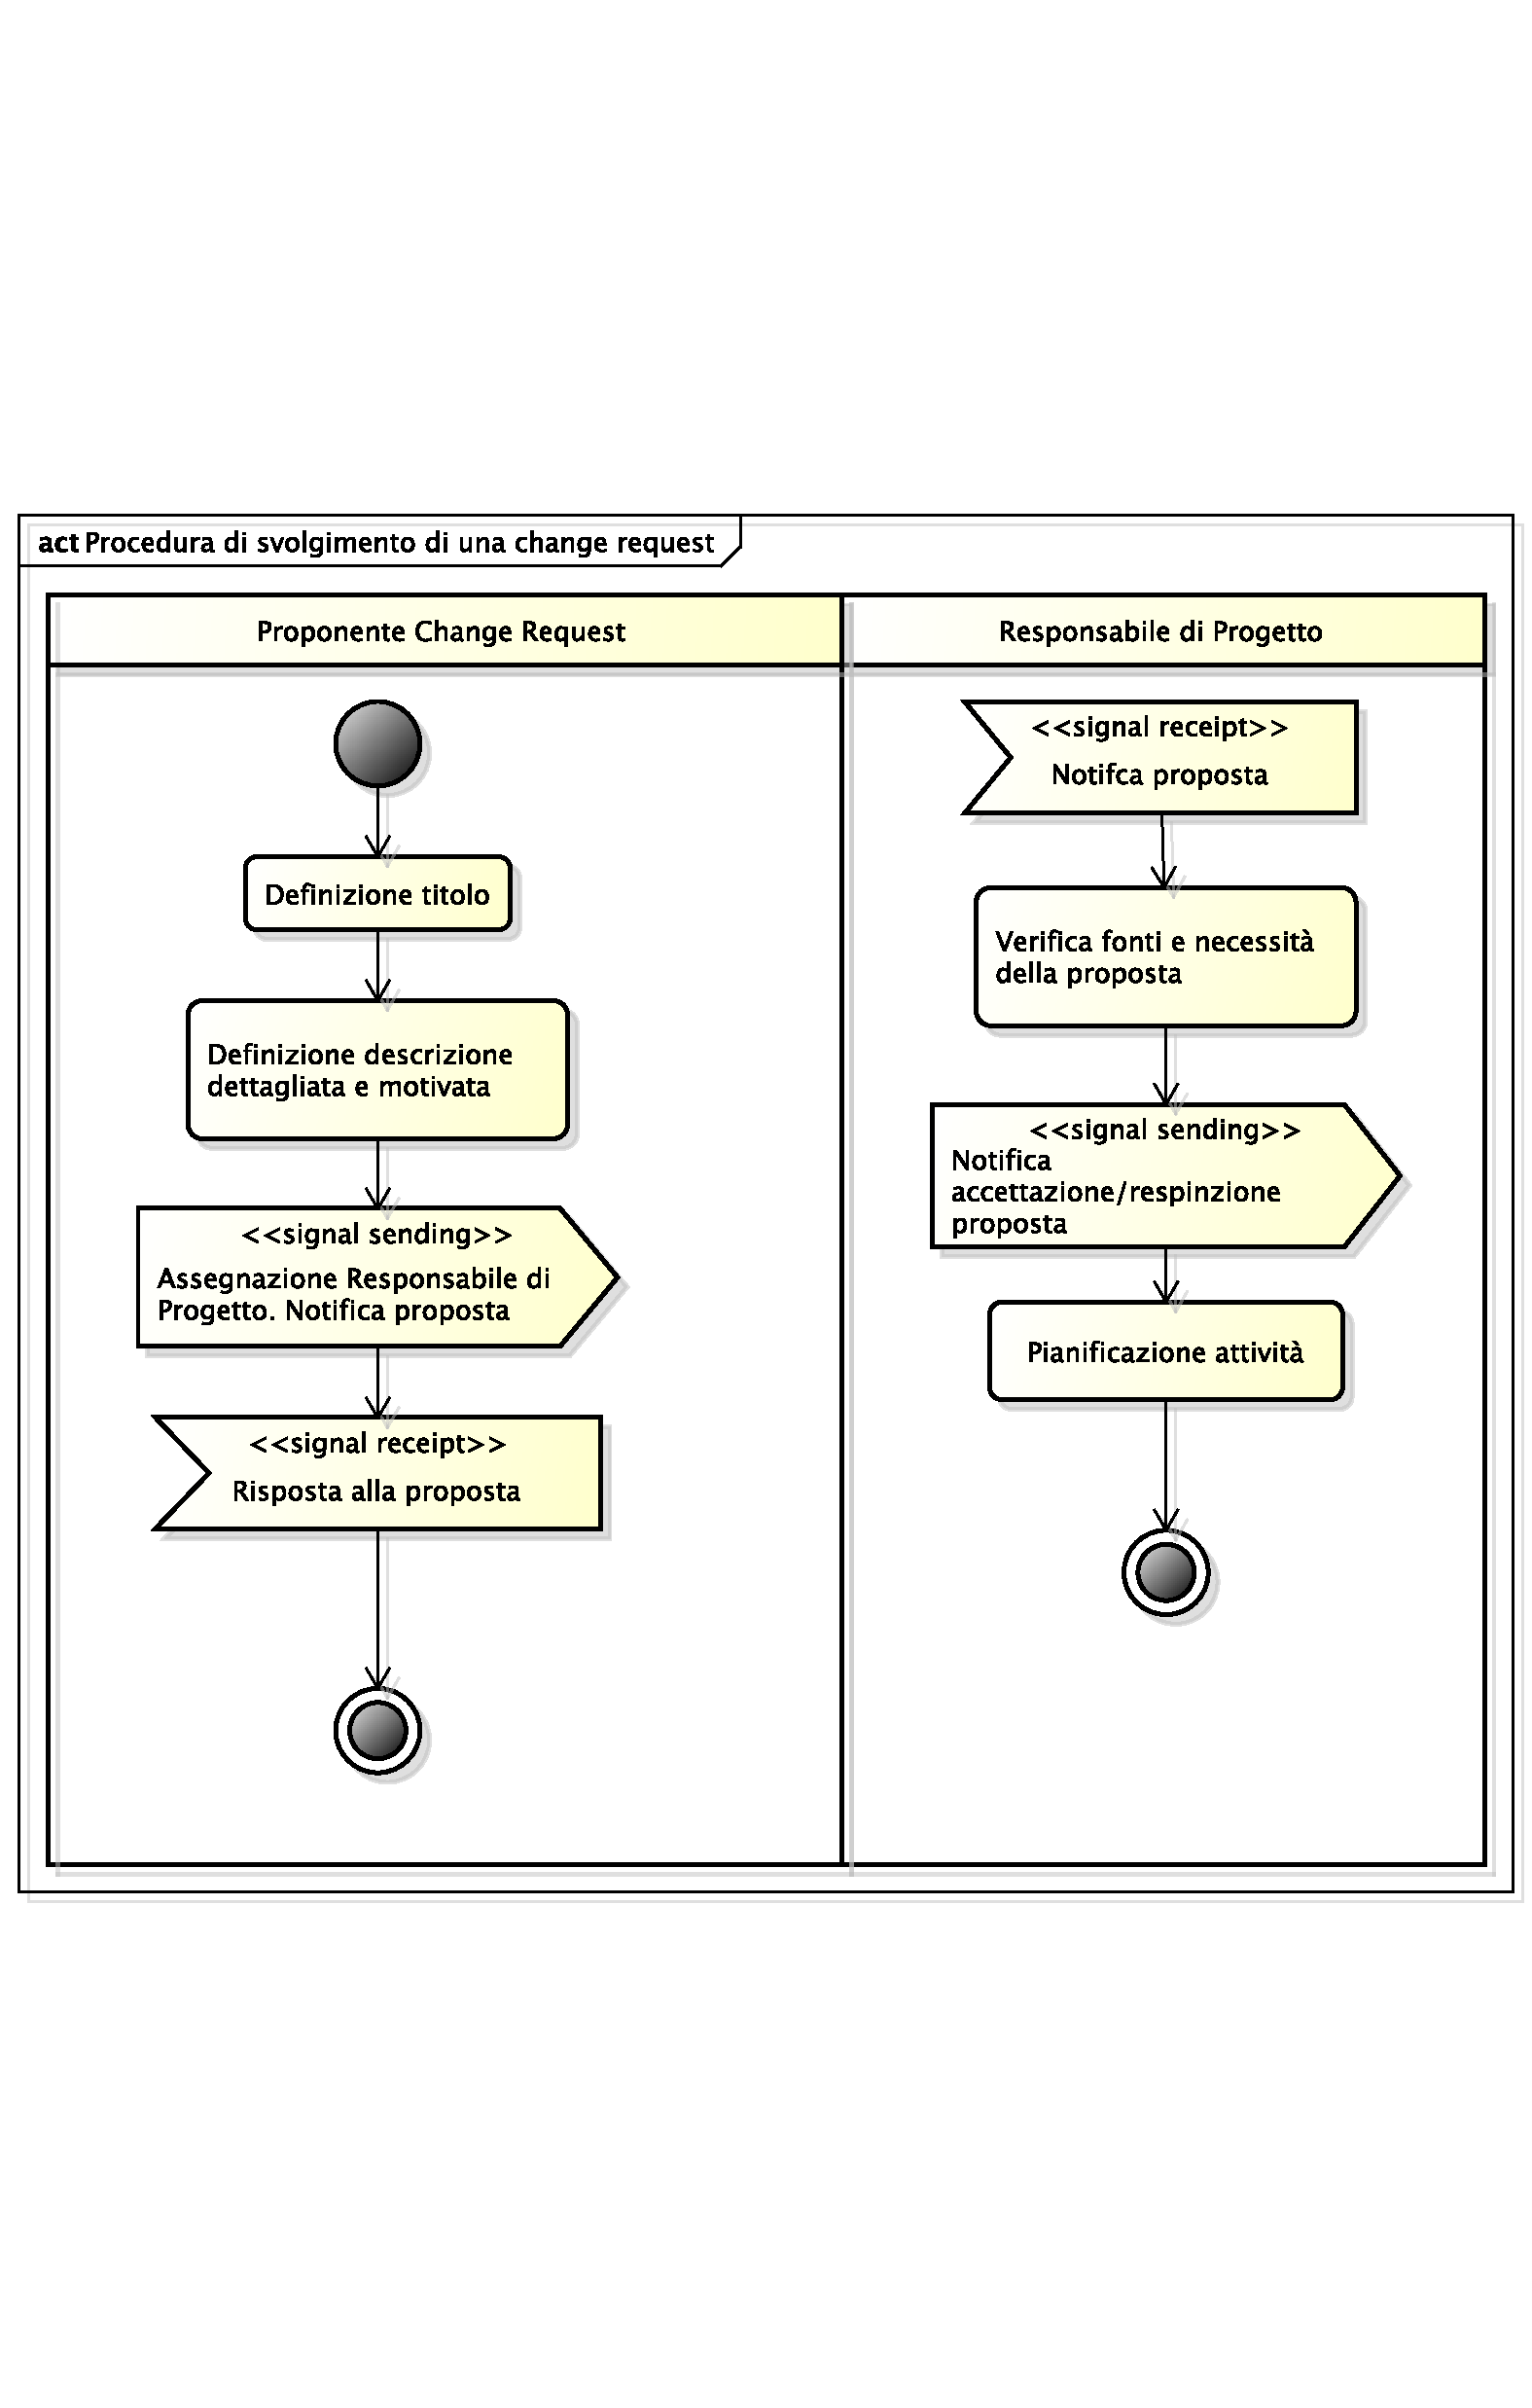
\includegraphics[width=14cm]{images/proc_change_request.pdf}
					\caption{Diagramma di attività - procedura di svolgimento di una change request}
					\label{fig:procedura_generazione_change_request}		
				\end{figure}
			
			\paragraph{Procedura di rilevazione dei rischi}
			Il \roleProjectManager{} ha il compito di individuare i rischi trovati nel \docNameVersionPdP. \\
			Questa attività è iterativa durante tutto il progetto e necessita di un continuo monitoraggio dei rischi rilevati nel periodo iniziale. Proprio per la sua natura non finita, si può andare in contro a problemi non previsti inizialmente. \\
			Qualora ciò avvenisse il \roleProjectManager{} dovrà eseguire la seguente sequenza di attività:
				\begin{enumerate}
					\item registrazione del riscontro effettivo dei rischi nel \docNameVersionPdP;
					\item pianificazione per la gestione dei nuovi rischi trovati;
					\item aggiornamento delle metodologie per fare fronte alla nuova pianificazione attuata;
					\item monitoraggio dei nuovi rischi riscontrati durante lo sviluppo del progetto.
				\end{enumerate}
				
		\subsubsection{Norme}
			\paragraph{Ruoli di Progetto}
			Lo sviluppo di un progetto necessita della collaborazione di diverse persone che andranno a ricoprire incarichi che rappresentano delle figure aziendali. \\
			Viene garantito che ogni componente del gruppo \groupName{} dovrà ricoprire, almeno una volta, tutti i ruoli. \\
			Questa rotazione potrebbe generare dei problemi dovuti a conflitti d'interesse in quanto lo stesso soggetto che svolge un compito potrebbe ritrovarsi a verificare l'operato svolto in precedenza. \\
			Un'attenta pianificazione da parte del \roleProjectManager{} dovrà preoccuparsi di non fare avvenire queste situazioni. \\
			Il compito di garantire che non siano stati fatti errori spetta al \roleVerifier, il quale, una volta riscontrata una incongruenza, dovrà notificarla al \roleProjectManager{} che avrà il compito di risolverla. \\ 
			Vengono ora presentati i diversi ruoli, delineandone le mansioni e le responsabilità.
				\subparagraph{Responsabile di Progetto}
				Il \roleProjectManager{} rappresenta il team e il progetto verso il committente e il proponente. \\
				Ha quindi le seguenti responsabilità e compiti:
					\begin{itemize}
						\item pianificazione e coordinamento delle attività;
						\item gestione e controllo delle risorse;
						\item analisi e gestione dei rischi;
						\item approvazione dell'offerta economica;
						\item assicurarsi che tutte le attività svolte siano conformi alle \docNameVersionNdP{} e rispettino la pianificazione effettuata nel \docNameVersionPdP;
						\item garantire che non ci siano conflitti di interesse. A tal proposito, se il \roleProjectManager{} dovesse prendere parte alla stesura di qualche documento, dovrà nominare un \roleProjectManager{} delegato che avrà il compito di sostituirlo nell'approvazione di quei documenti;
						\item redigere il \docNameVersionPdP.
					\end{itemize}
					
				\subparagraph{Amministratore}
				L'\roleAdministrator{} è il responsabile dell'ambiente di lavoro. \\
				Ha quindi il compito di:
					\begin{itemize}
						\item ricercare e implementare strumenti che automatizzino il maggior numero di operazioni;
						\item gestire il versionamento del codice e della documentazione di progetto;
						\item fornire procedure che servono a garantire la qualità del prodotto uscente da un determinato compito;
						\item redigere le \docNameVersionNdP.
					\end{itemize}
				\subparagraph{Analista}
				L'\roleAnalyst{} è il responsabile dell'attività di analisi.\\
				Ha quindi il compito di:
					\begin{itemize}
						\item comprendere a pieno la natura del problema e la sua complessità;
						\item ricercare i requisiti che servono per realizzare il prodotto richiesto dal proponente;
						\item redigere lo \docNameVersionSdF;
						\item redigere l'\docNameVersionAdR.
					\end{itemize}
				\subparagraph{Progettista}
				Il \roleDesigner{} è il responsabile delle attività di progettazione. \\
				Ha quindi il compito di:
					\begin{itemize}
						\item effettuare scelte progettuali estratte da soluzioni note e fortemente testate (design pattern);
						\item effettuare scelte progettuali che permettano al sistema di essere il più facilmente mantenibile in futuro;
						\item produrre una soluzione comprensibile, attuabile e motivata;
						\item redigere il \docNameVersionPdQ.
					\end{itemize}
				\subparagraph{Programmatore}
				Il \roleProgrammer{} è il responsabile delle attività di codifica necessarie a portare il prodotto in uno stato che riesca a soddisfare i requisiti richiesti. Deve inoltre programmare i componenti che servono a verificare il sistema. \\
				Ha quindi il compito di:
					\begin{itemize}
						\item scrive codice che rispetti le metriche stabilite per la sua scrittura;
						\item implementare lo soluzione descritte dal \roleDesigner;
						\item implementare i test sul codice prodotto.
					\end{itemize}
				\subparagraph{Verificatore}
				Il \roleVerifier{} è il responsabile delle attività di verifica. \\
				Ha quindi il compito di:
					\begin{itemize}
						\item controllare la conformità di ogni stadio del ciclo di vita del prodotto;
						\item garantire che le attività svolte siano conformi alle norme stabilite;
						\item redige il \docNameVersionPdQ{} per la parte che illustra l'esito e la completezza delle verifiche effettuate.
					\end{itemize}
		
			\paragraph{Formato dei task}
			\label{par:formato_dei_task}
			I task che si andranno ad aprire devono contenere le seguente informazioni:
				\begin{itemize}
					\item \textbf{Titolo}: una breve descrizione del compito da eseguire;
					\item \textbf{Descrizione}: qualora non fosse abbastanza esaustivo il titolo del task, si deve fornire una descrizione più dettagliata dell'attività da svolgere;
					\item \textbf{Data di scadenza}: la data entro la quale dovrà essere svolto il lavoro;
					\item \textbf{Assegnatario}: il membro del team che dovrà eseguire il task indicato;
					\item \textbf{Verificatore}: il membro del team che andrà ad eseguire la verifica sull'operato svolto dall'assegnatario;
					\item \textbf{Followers}: i membri del team che si vuole rendere partecipi sull'attività svolta. Dovrà essere sempre aggiunto l'utente ``MainMashUp''.
				\end{itemize}
			\noindent
			La figura \ref{fig:template_task_asana} illustra come vengono rappresentate queste informazioni su Asana. Inoltre l'immagine viene proprio presa da uno screenshot di un template di task, copiabile dal \roleProjectManager{} e modificabile una volta copiato a seconda dell'esigenze riportate in precedenza.
				\begin{figure}[htbp]
					\centering
					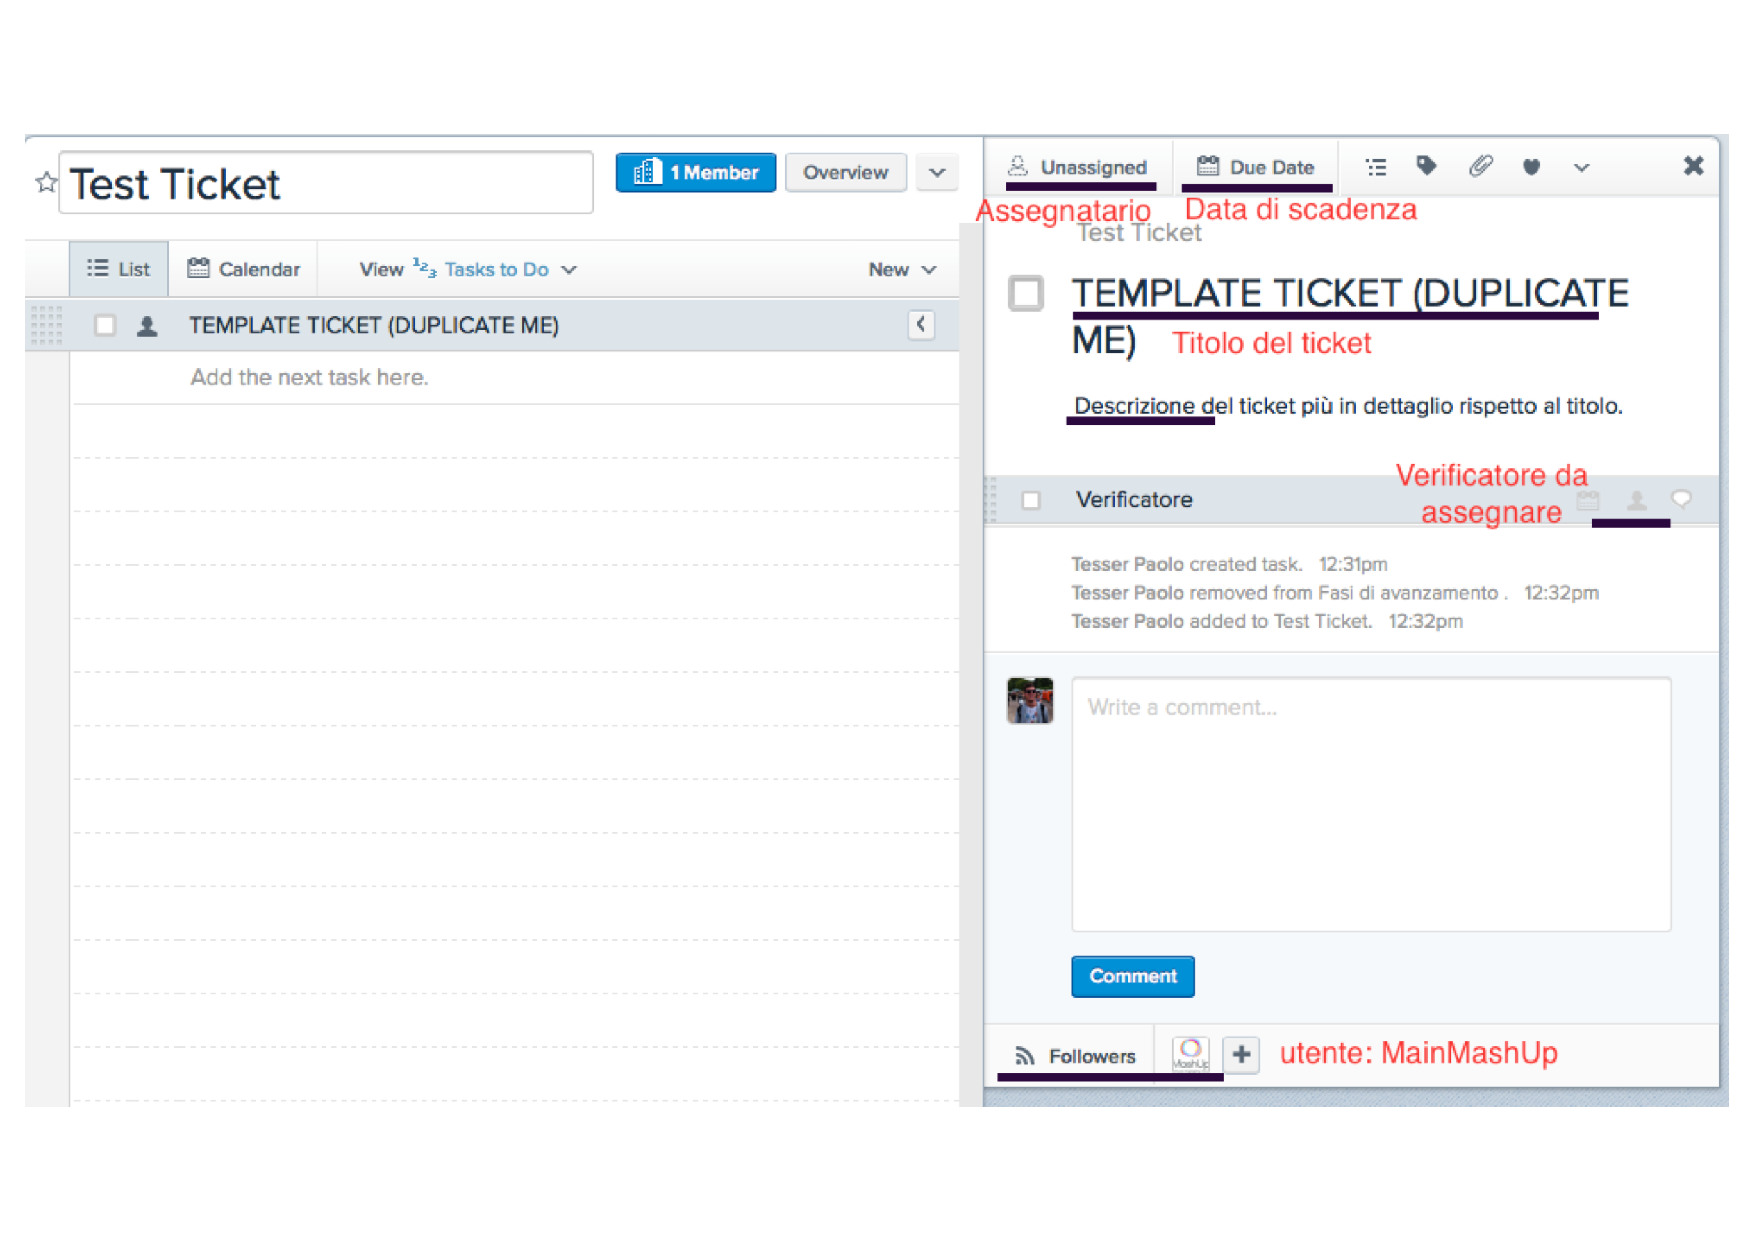
\includegraphics[width=14cm]{images/tpl_task_asana.pdf}
					\caption{Template Task su Asana}
					\label{fig:template_task_asana}
				\end{figure}
			
			\paragraph{Formato delle change request} 
			(NOTA: DA SPOSTARE NEL PROCESSO DI SUPPORTO -> Risoluzione di Problemi) \\
			Le change request che si andranno ad aprire devono contenere le seguente informazioni:
				\begin{itemize}
					\item \textbf{Titolo}: una breve descrizione di cosa si vorrebbe cambiare;
					\item \textbf{Descrizione}: una descrizione più dettagliata del cambiamento, motivando opportunamente la necessità riscontrata;
					\item \textbf{Assegnatario}: il \roleProjectManager{} al momento in carica secondo la rotazione dei ruoli;
					\item \textbf{Proponente}: chi è stato a proporre questo cambiamento. Sarà di fatto chi ha aperto la richiesta.
				\end{itemize}
			\noindent
			La figura \ref{fig:template_change_request_asana} illustra come vengono rappresentate queste informazioni su Asana. Inoltre l'immagine viene proprio presa da uno screenshot di un template di una change request, copiabile da qualunque membro desideri proporre un cambiamento e modificabile una volta copiato a seconda dell'esigenze riportate in precedenza.
				\begin{figure}[htbp]
					\centering
					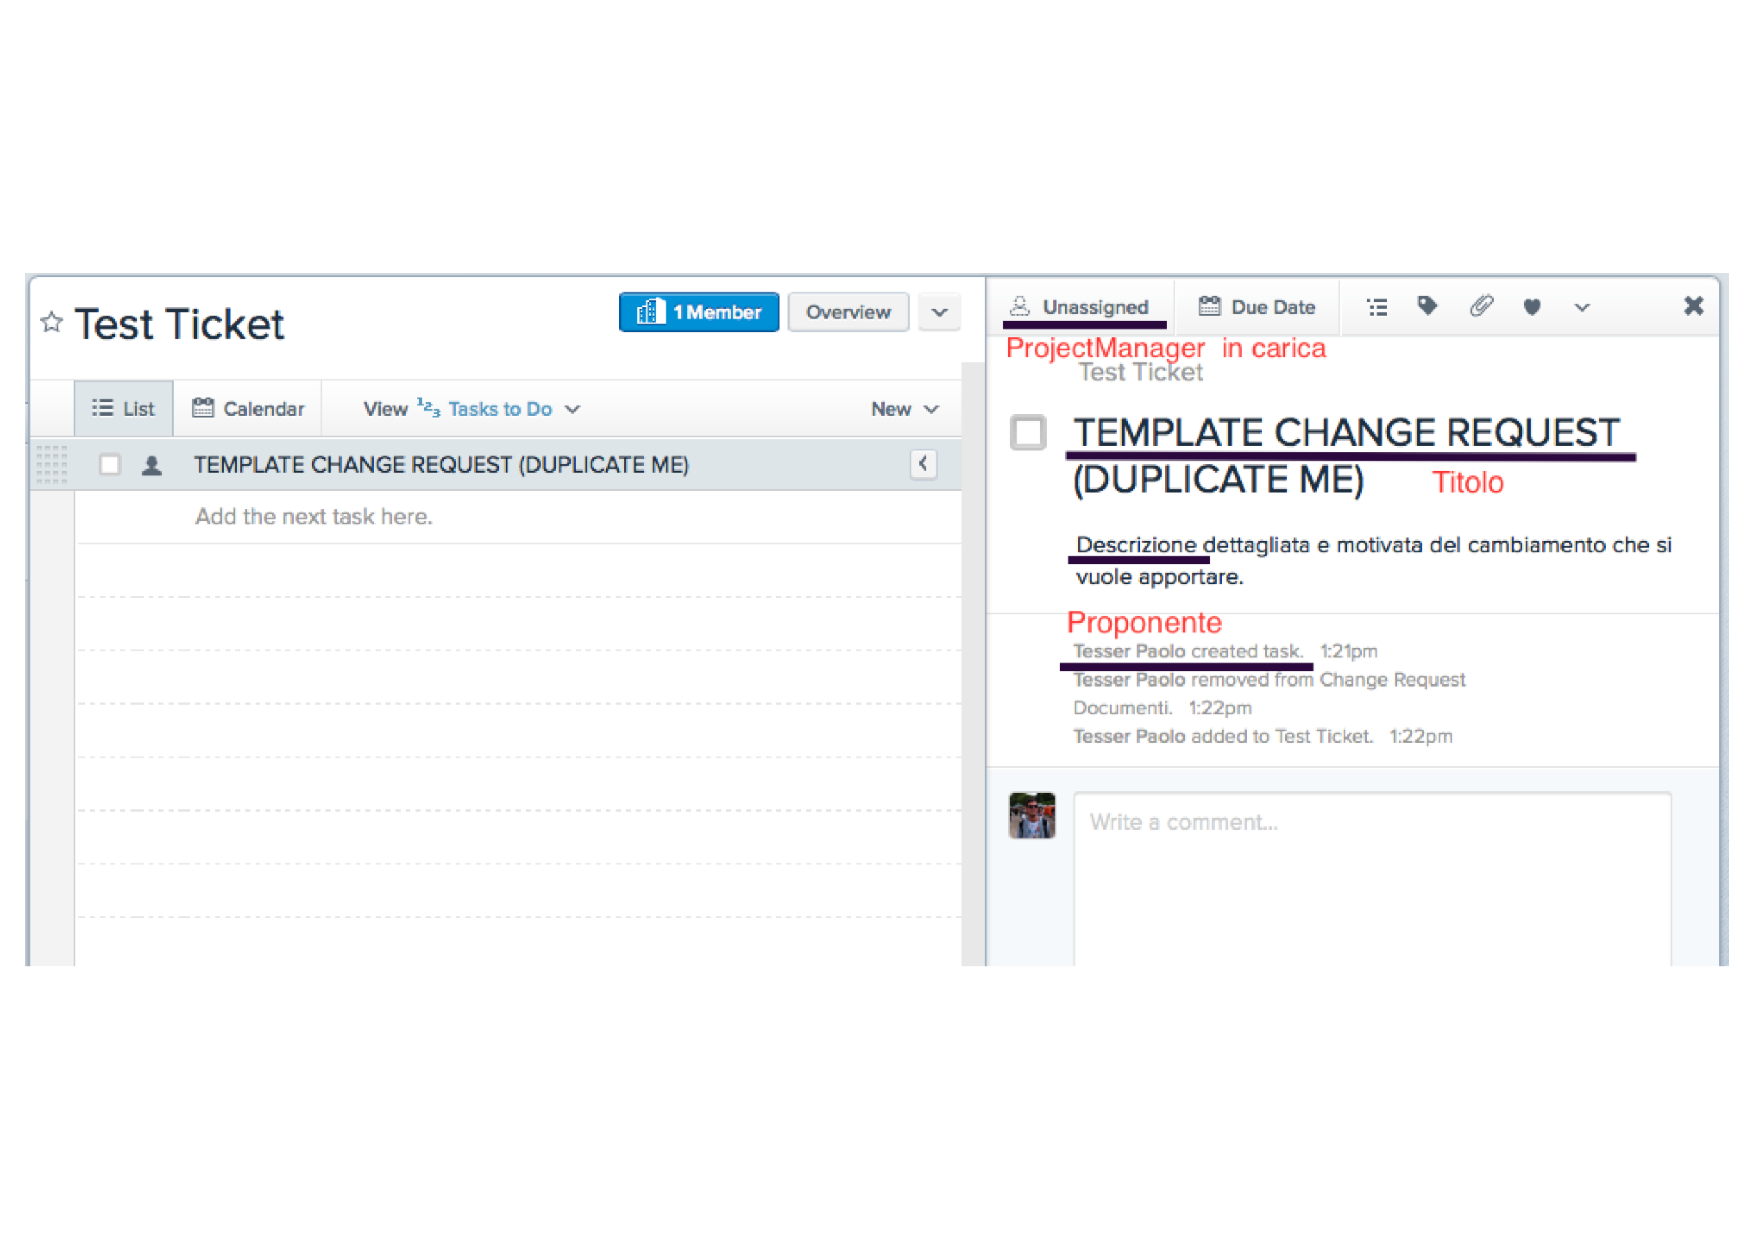
\includegraphics[width=14cm]{images/tpl_change_request_asana.pdf}
					\caption{Template Change Request su Asana}
					\label{fig:template_change_request_asana}
				\end{figure}
	
		\subsubsection{Strumenti}
			\paragraph{Asana}
			\label{sec:asana}
			Asana è l'applicazione web scelta per la gestione dei task.\\
			Registrandosi con una mail di dominio personale come quella riportata nella sezione \ref{sec:mail} è possibile usufruire di maggiori servizi che consentono una più facile gestione del team da parte del \roleProjectManager.
			\paragraph{Astah}
			Astah è l'applicativo scelto per la creazione di grafici UML.
			La versione adottata è quella Professional, resa disponibile con una licenza gratuita per gli studenti dei corsi universitari registrandosi tramite l'indirizzo:
				\begin{center}
					nome.cognome.X@studenti.unipd.it
				\end{center}

			\paragraph{ProjectLibre}
			ProjectLibre è il prodotto scelto per la realizzazione dei diagrammi di Gaant e quelli di PERT.
			\paragraph{NetSons}
			NetSons è il servizio di hosting che il team ha deciso di adottare a scopo principalmente formativo. \\
			Il dominio creato è:
				\begin{center}
					\url{http://www.mashup-unipd.it}
				\end{center}
			Il servizio fornisce anche una serie di email personali che il gruppo ha deciso di utilizzare come spiegato nelle sezioni \ref{sec:mail} e \ref{sec:comunicazioni_esterne}.
			\paragraph{Skype}
			Skype è l'applicativo scelto per effettuare videochiamate o chiamate VoIP tra i componenti del gruppo quando c'è la necessità di consultarsi o risolvere problemi e non è possibile essere presenti fisicamente nello stesso ambiente.		
			\paragraph{WhatsApp}
			WhatsApp è l'applicativo di messaggistica scelto per le comunicazioni interne e informali al gruppo.
			\paragraph{TO DO - Strumento per la Presentazione}
			TO DO


	\subsection{Gestione delle Infrastrutture}
	
		\subsubsection{Attività}
			\paragraph{Gestione del Repository}
			Il gruppo ha deciso di utilizzare due repository che servono a svolgere funzioni diverse, ma necessarie, allo sviluppo del sistema finale. \\
			Il servizio di hosting scelto consente, tramite licenza ``educational'', di impostare la visibilità degli ambienti come privata. \\
			Una volta iscritti i membri dovranno comunicare all'\roleAdministrator{} il loro nome utente che provvederà ad autorizzarne l'accesso.
				\begin{itemize}
					\item \textbf{doc\_BDSM\_App}: gestione della documentazione;
					\item \textbf{src\_BDSM\_App}: gestione del codice;
				\end{itemize}
			\paragraph{Gestione dei Git Hooks}
			L'\roleAdministrator{} ha il compito di mantenere gli script che permettono di tenere il repository consistente con le norme descritte in questo documento. \\
			Questo strumento per sua natura ha dei limiti, in quanto deve essere installato localmente in ogni macchina da parte dei singoli membri. \\
			L'\roleAdministrator{} provvederà a notificare ai membri del gruppo quando applicare la procedura descritta nella sezione \ref{sec:installazione_git_hooks} tramite i sistemi visti nella sezione \ref{sec:comunicazioni_interne}. \\
			La notifica potrà avvenire principalmente in due casi:
				\begin{itemize}
					\item ogni volta che un membro clona il repository in locale nella sua macchina;
					\item ogni volta che l'\roleAdministrator{} effettua un aggiornamento degli script.
				\end{itemize}
				
			\paragraph{Gestione del template del messaggio di commit}
			L'\roleAdministrator{} ha il compito di mantenere il meno ambiguo possibile l'ambiente di lavoro. \'E per questo che si è deciso di utilizzare un template standard per andare a scrivere il messaggio della commit.
			Questo strumento per sua natura ha dei limiti, in quanto deve essere installato localmente in ogni macchina da parte dei singoli membri. \\
			L'\roleAdministrator{} provvederà a notificare ai membri del gruppo quando applicare la procedura descritta nella sezione \ref{sec:installazione_msg_commit} tramite i sistemi visti nella sezione \ref{sec:comunicazioni_interne}. \\
			La notifica potrà avvenire principalmente in due casi:
				\begin{itemize}
					\item la prima volta che un membro entra a fare parte del team di lavoro;
					\item ogni volta che l'\roleAdministrator{} effettua un aggiornamento degli script.
				\end{itemize}
				
				
		\subsubsection{Procedure}
			\paragraph{Installazione e manutenzione Git Hooks}
			\label{sec:installazione_git_hooks}
			I membri del team dovranno eseguire questa procedura una volta ricevuta la notifica da parte dell'\roleAdministrator. \\
			Il diagramma presente nella figura \ref{fig:installazione_git_hook} illustra in maniera più schematizzata i compiti da eseguire.
				\begin{enumerate}
					\item entrare dalla root del repository tramite terminale nella cartella ``script'';
					\item digitare sempre da terminale il comando:
						\begin{center}
							make hook
						\end{center}
				\end{enumerate}
						
			\begin{figure}[htbp]
				\centering
				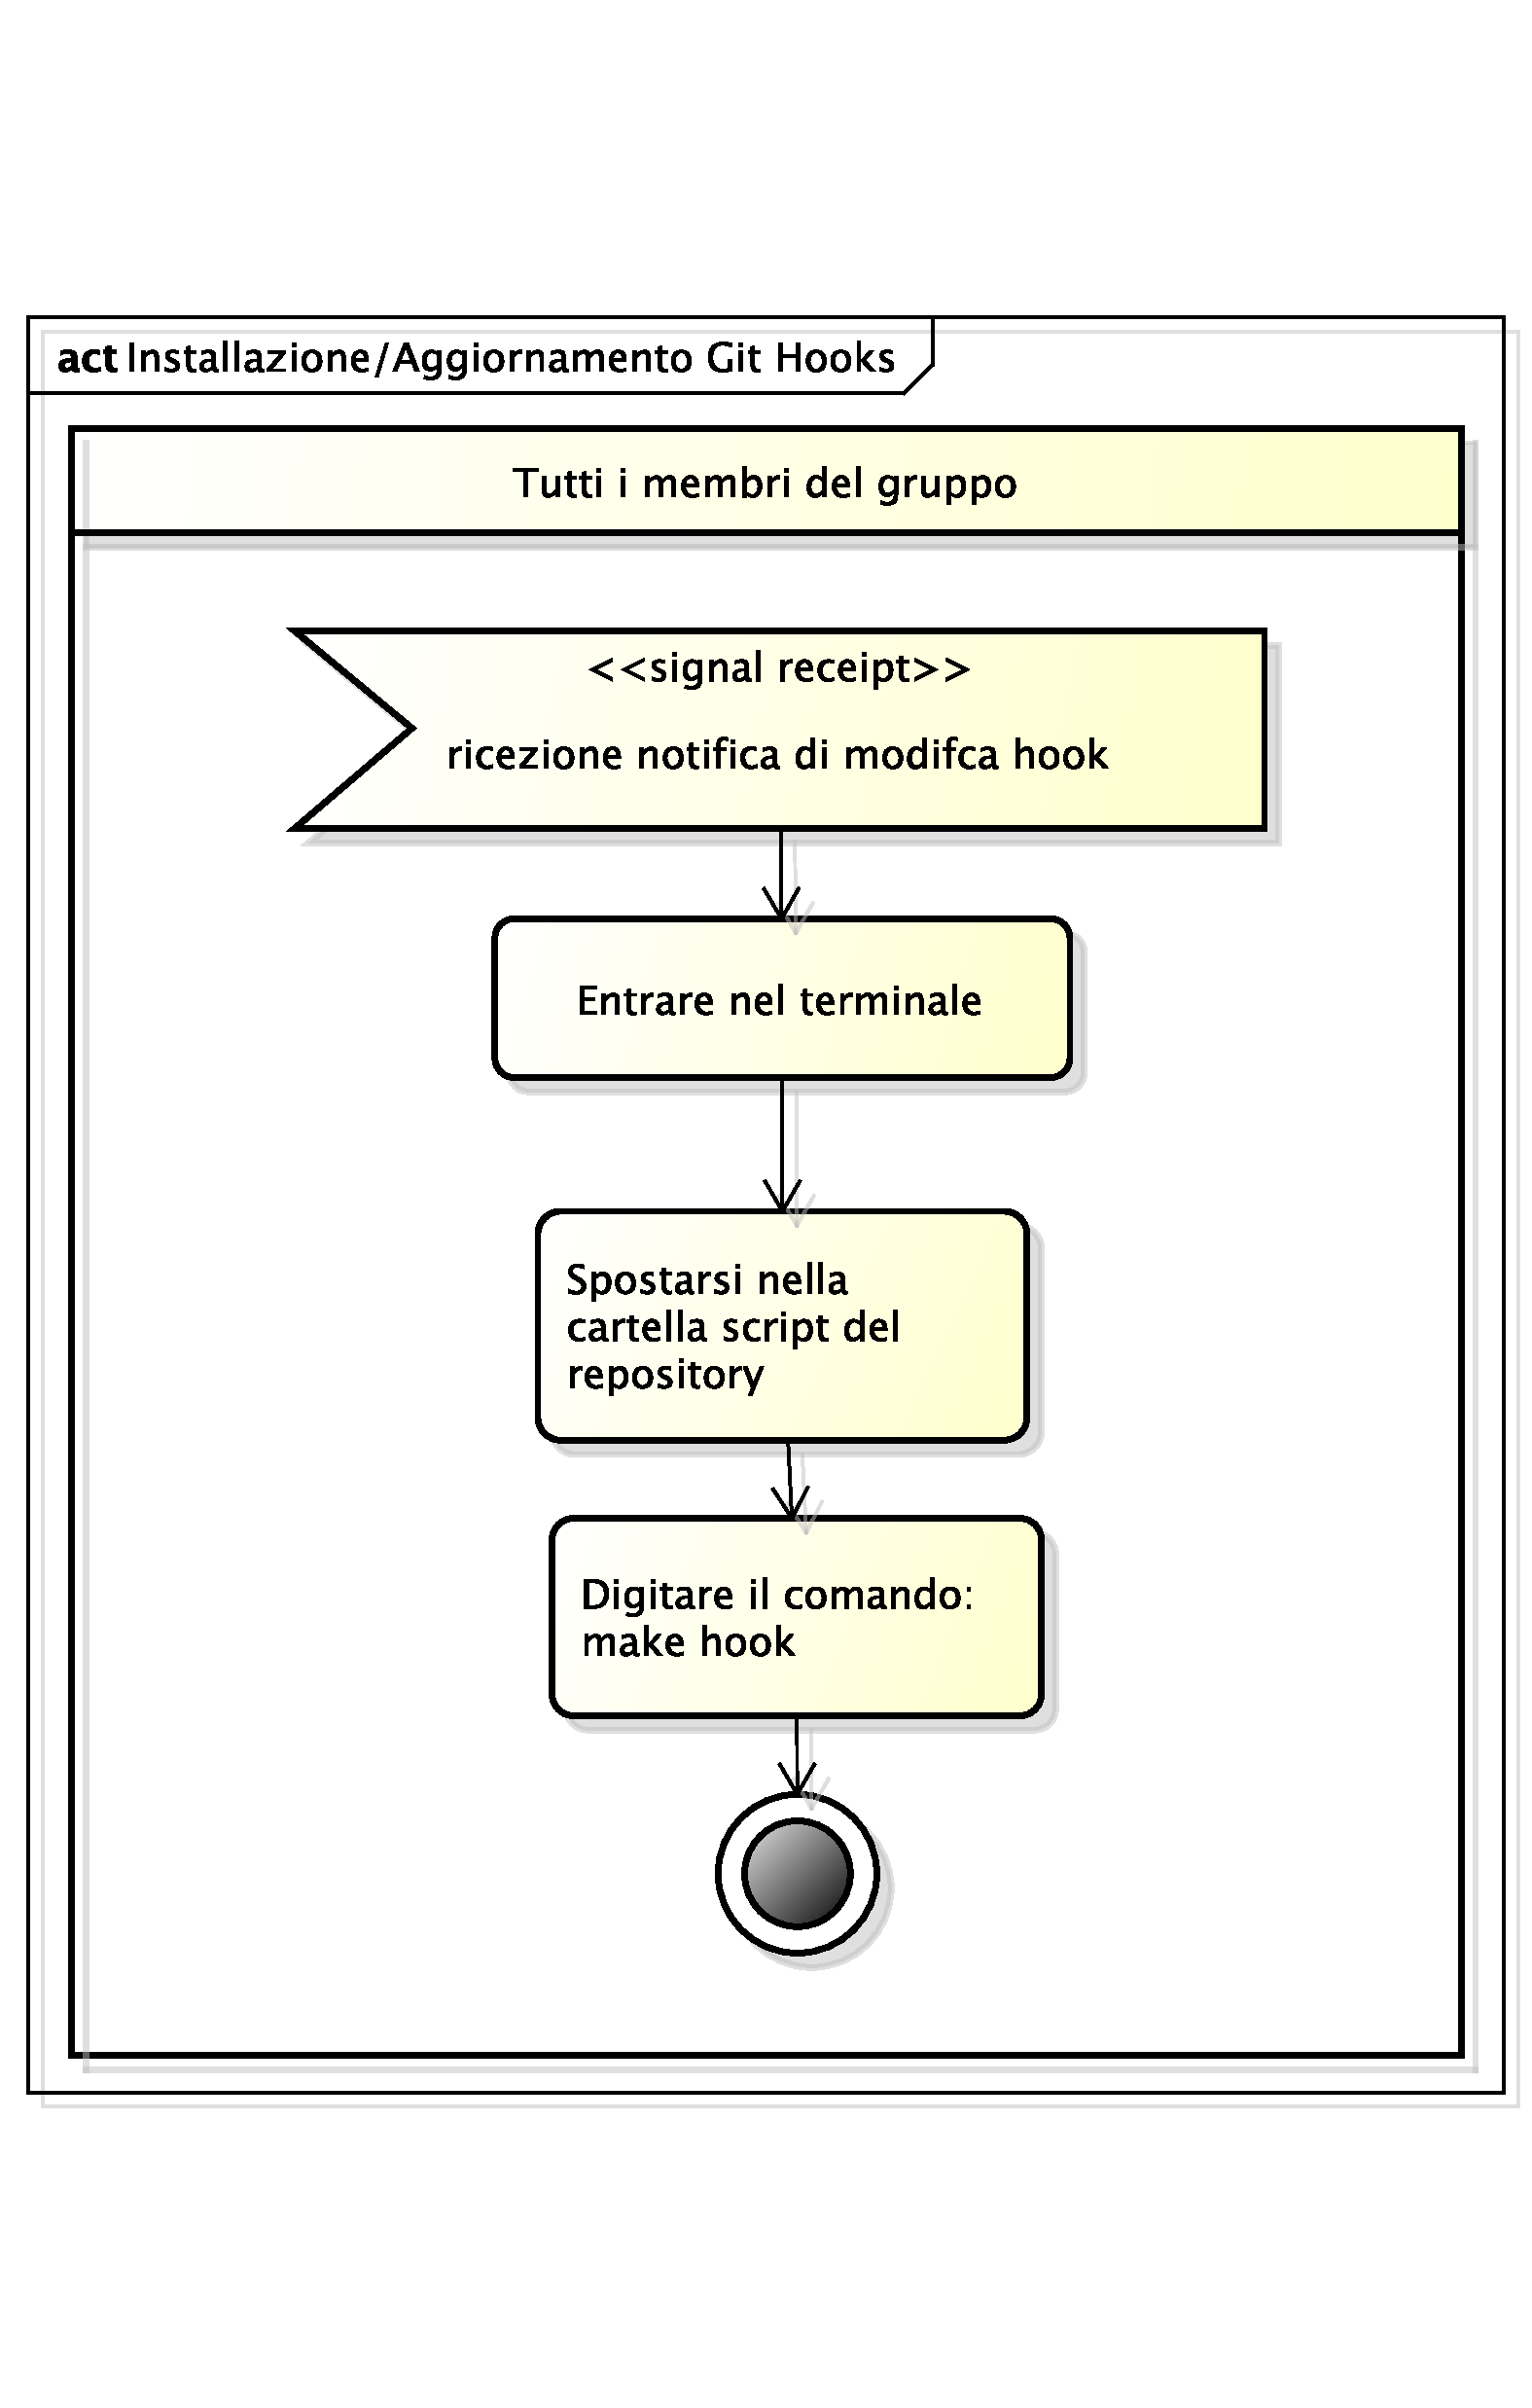
\includegraphics[width=11cm]{images/inst_git_hook.pdf}
				\caption{Diagramma di attività - installazione/aggiornamento dei Git Hooks}
				\label{fig:installazione_git_hook}
			\end{figure}
			
			\paragraph{Installazione e manutenzione messaggio di commit}
			\label{sec:installazione_msg_commit}
			I membri del team dovranno eseguire questa procedura una volta ricevuta la notifica da parte dell'\roleAdministrator. \\
			Il diagramma presente nella figura \ref{fig:installazione_msg_commit} illustra in maniera più schematizzata i compiti da eseguire.
				\begin{enumerate}
					\item scaricare il nuovo template allegato alla notifica ricevuta che avrà nome ``gitmessage.txt'';
					\item se è la prima volta che si esegue la procedura, lanciare il seguente comando dal terminale, altrimenti passare al passo successivo:
						\begin{center}
							git config --global core.editor ``mate''
						\end{center}
					\noindent
					Sostituite ``mate'' con l'editor che preferite;
					\item entrare nella directory principale dell'utente (esempio: /Users/nomeutente);
					\item copiare il file allegato in questa cartella rinominandolo in modo da renderlo nascosto inserendo un punto davanti al nome (esempio: .gitmessage.txt).
				\end{enumerate}
				
			\begin{figure}[htbp]
				\centering
				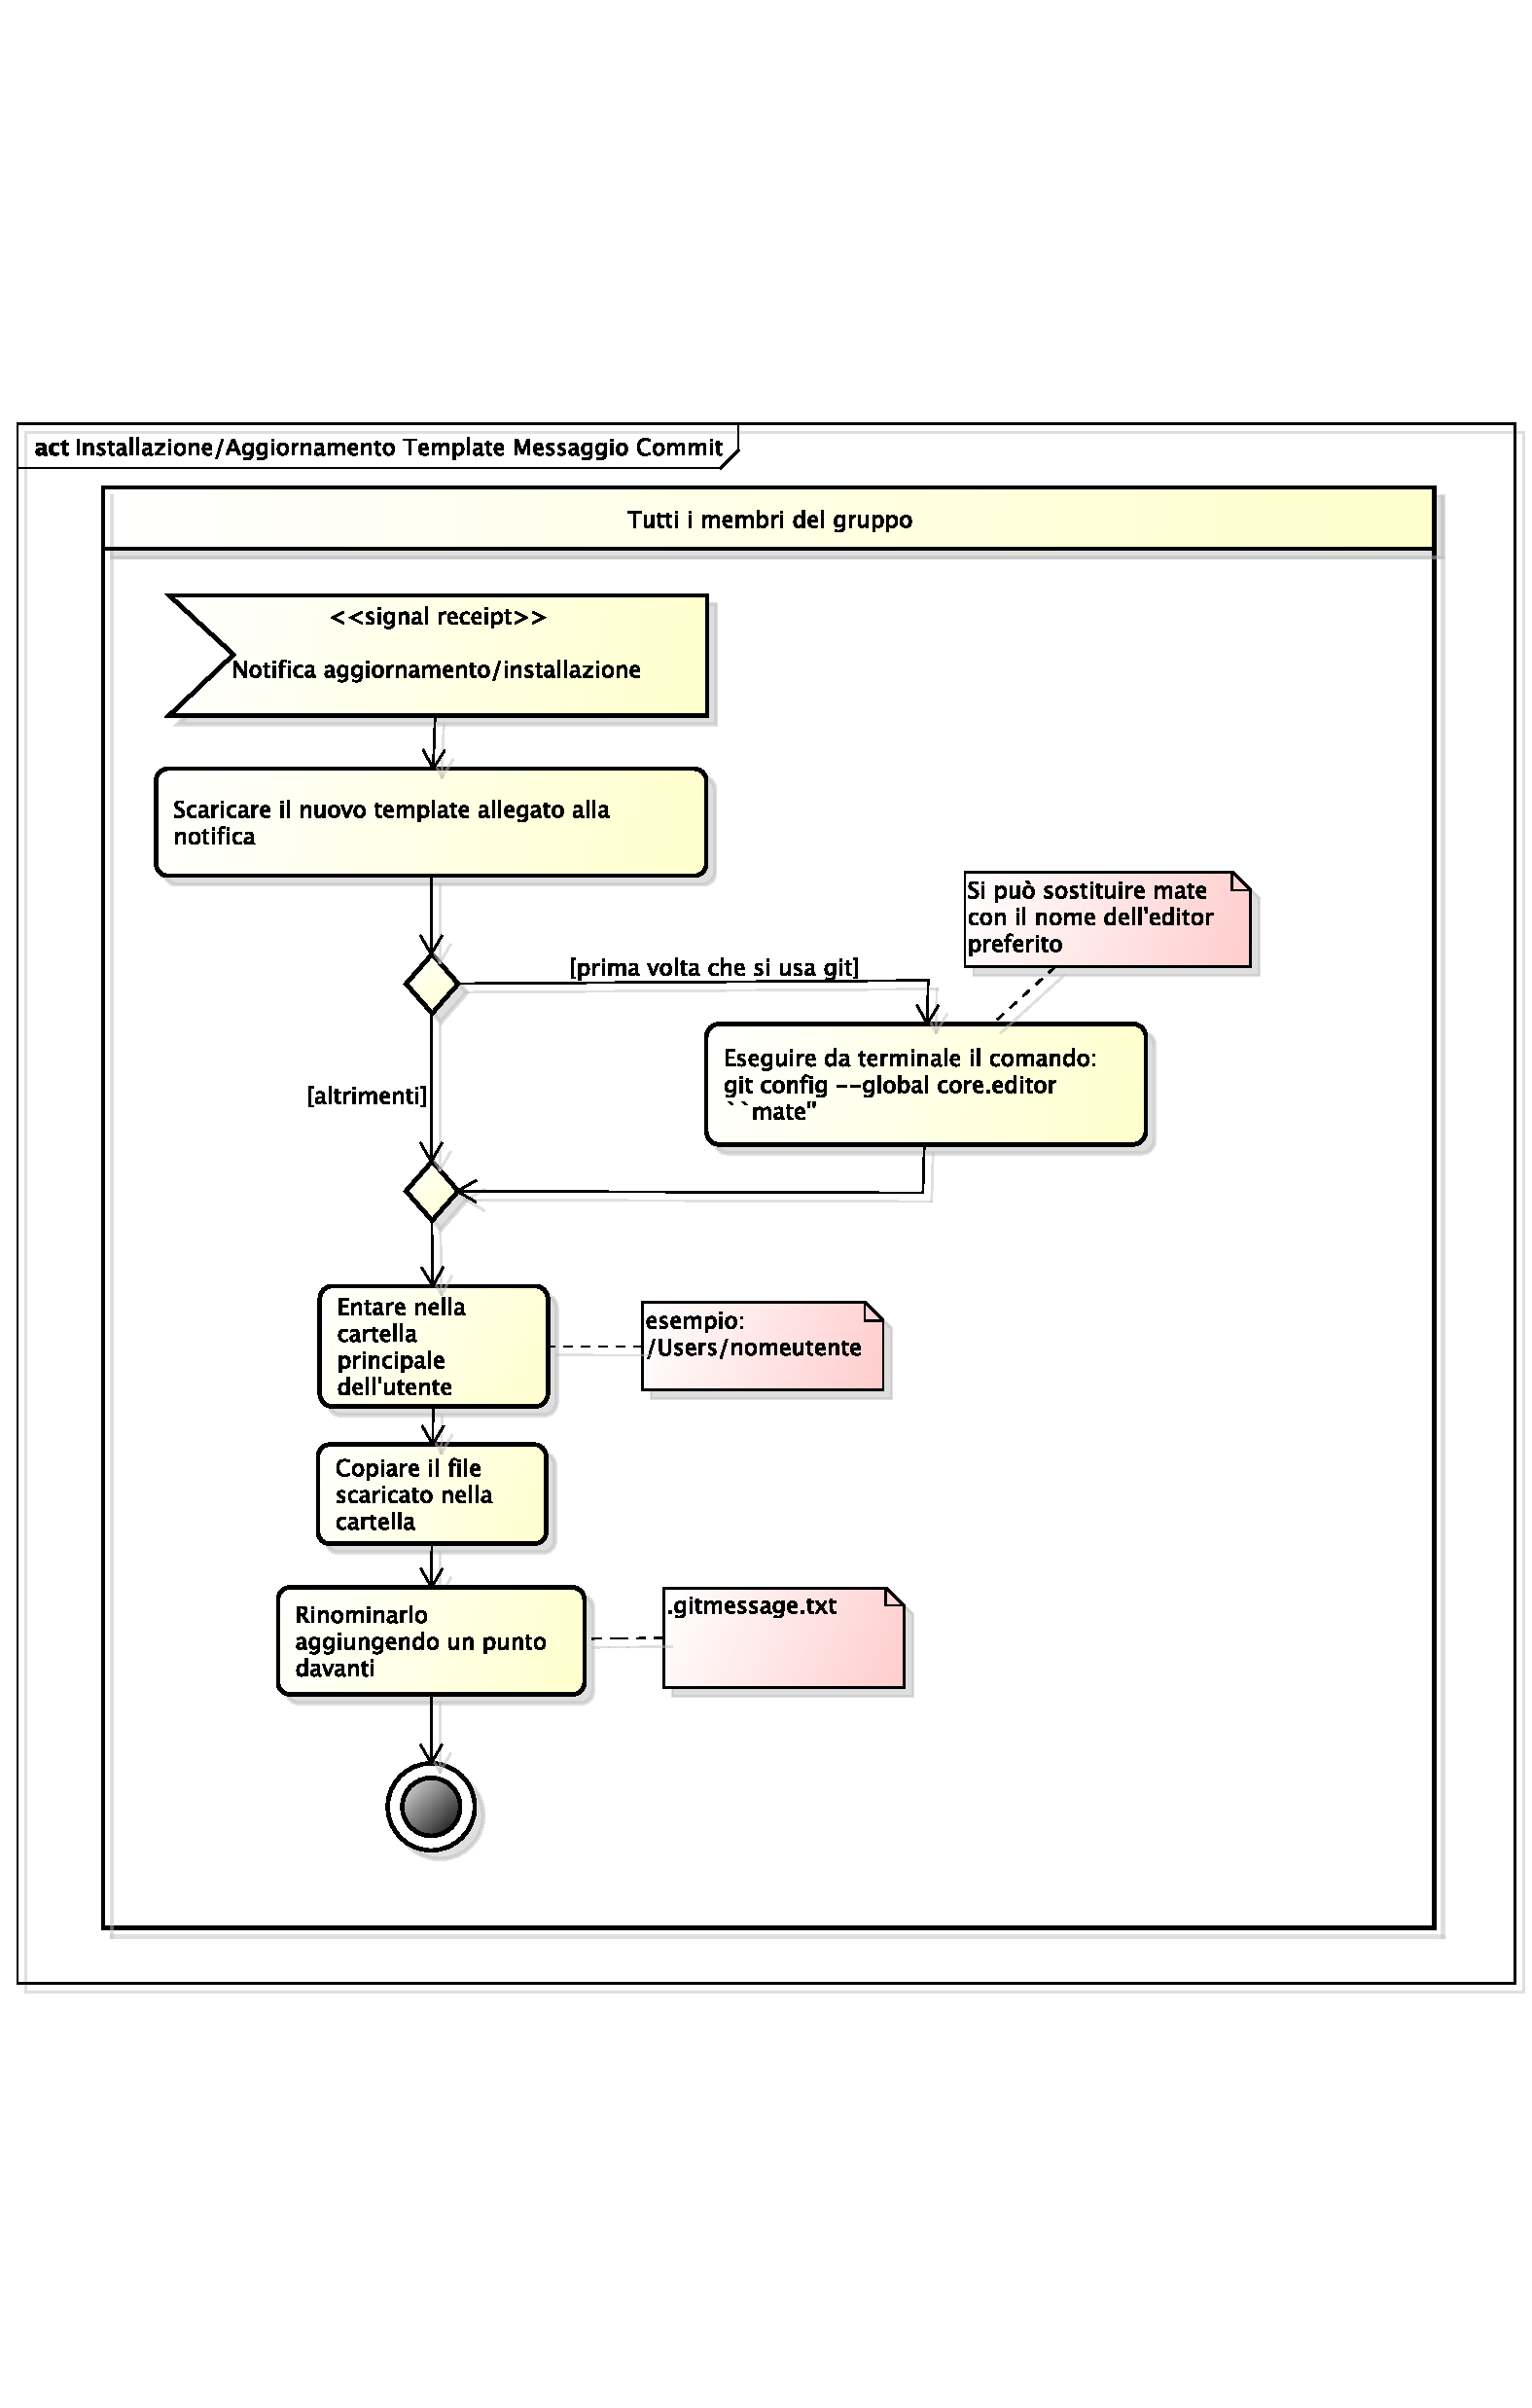
\includegraphics[width=14cm]{images/inst_tpl_commit_msg.pdf}
				\caption{Diagramma di attività - installazione/aggiornamento del template del messaggio per la commit}
				\label{fig:installazione_msg_commit}
			\end{figure}
			
		\subsubsection{Norme}
			\paragraph{Repository}
				\subparagraph{Nomi dei file in doc\_BDSM\_App}
				I file e le cartelle presenti nel repository devono essere conformi al seguente formalismo tratto dallo Standard ISO 9660:1999 (Level 2):
					\begin{itemize}
						\item i caratteri usati sono solo quelli minuscoli a-z, 0-9, l'underscore (\_) e il punto (.) (esempio: nome\_del\_documento.tex);
						\item non sono ammessi caratteri accentati;
						\item i nomi non possono includere spazi o finire con un punto (.);
						\item i nomi non devono contenere più di un punto (.) ad eccezione di quelli che fanno riferimento ad una specifica versione (esempio: studio\_di\_fattibilita\_v1.0.0.pdf);
						\item i nomi non devono essere più lunghi di 21 caratteri esclusi i 3 destinati all'estensione.
					\end{itemize}

				\subparagraph{Struttura di doc\_BDSM\_App}
				Le cartelle nel repository verranno organizzate nel seguente modo a partire dalla root:
					\begin{itemize}
						\item \textbf{consegne}: contenente i documenti finali con anche la versione da consegnare alle diverse revisioni. Sono presenti le cartelle:
							\begin{itemize}
								\item \textbf{revisione\_dei\_requisiti}: contenente i documenti necessari alla revisione dei requisiti;
								\item \textbf{revisione\_di\_progettazione}: contenente i documenti necessari alla revisione di progettazione;
								\item \textbf{revisione\_di\_qualifica}: contenente i documenti necessari alla revisione di qualifica;
								\item \textbf{revisione\_di\_accettazione}: contenente i documenti necessari alla revisione di accettazione.
							\end{itemize}
						\noindent
						All'interno di ciascuna di esse ci sarà un'ulteriore suddivisione in due categorie:
							\begin{itemize}
								\item \textbf{interni}: contenente i documenti necessari al gruppo per la sua organizzazione;
								\item \textbf{esterni}: contenente i documenti necessari alla pianificazione e all'avanzamento dello sviluppo.
							\end{itemize}
							
						\item \textbf{documenti}:
							\begin{itemize}
								\item \textbf{template}: contenente i file che servono per gestire in maniera univoca la redazione di un documento;
								\item \textbf{template\_document}: contenente i file di esempio che dovranno essere utilizzati per ogni documento reale;
								\item una cartella per ogni documento che avrà come nome quello del documento in questione (esempio: norme\_di\_progetto).
							\end{itemize}
							
						\item \textbf{script}: contenente tutti gli script necessari ad automatizzare il lavoro e il controllo della documentazione.
					\end{itemize}
					
				\subparagraph{Nomi dei file in src\_BDSM\_App}
				La presente sezione verrà redatta in futuro, presumibilmente nella prima fase di progettazione di dettaglio e codifica dei requisiti come esposto nel documento \docNameVersionPdP.
				\subparagraph{Struttura di src\_BDSM\_App}
				La presente sezione verrà redatta in futuro, presumibilmente nella prima fase di progettazione di dettaglio e codifica dei requisiti come esposto nel documento \docNameVersionPdP.

				\subparagraph{Modello di sviluppo}
				Per lo sviluppo della documentazione e del codice necessari al progetto si è scelto di adottare il modello proposto dal proponente, spiegato nel dettaglio al seguente link:
					\begin{center}
						\url{http://nvie.com/posts/a-successful-git-branching-model/}
					\end{center}
					Ogni membro del gruppo dovrà leggere l'articolo e applicarlo secondo le norme di denominazione dei branch presenti in esso.

				\subparagraph{Template messaggio di commit}
				\label{sec:messaggio_di_commit}
				Il messaggio di commit dovrà essere conforme alla seguente notazione:
					\begin{verbatim}
						Title:
						Desc:
						Task: Reported in #id_task
						Option: [option][option]
						END
					\end{verbatim}
				% \lstnewenvironment{testo}[1][]
				% {
				%	\lstset{
				%		basicstyle=\small\ttfamily, 
				%		columns=fullflexible,
				%		keywordstyle=\color{red}\bfseries, 
				%		commentstyle=\color{blue},
				%		language=C++, % non importa il linguaggio in questo caso perchè è solo testo
				%		basicstyle=\small,
				%		numbers=left,
				%		numberstyle=\tiny,
				%		stepnumber=1,
				%		numbersep=5pt,
				%		frame=shadowbox,
				%		#1
				%	}
				% }{}
				
				% \begin{testo}[caption={Template messaggio di commit}]
				%	Title:
				%	Desc:
				%	Task: Reported in #id_task
				%	Option: [option][option]
				%	END
				% \end{testo}
				
					\begin{itemize}
						\item \textbf{Title}: inserire una breve descrizione come titolo di quello che è stato fatto (massimo 43 caratteri);
						\item \textbf{Desc}: inserire una descrizione più esaustiva dell'attività svolta qualora non fosse sufficiente quella data nel titolo;
						\item \textbf{Task}: al posto della dicitura ``id\_task'' inserire l'id del task effettivo reperibile su Asana secondo le modalità esposte nella sezione \ref{par:procedura_reperimento_id_task_asana};
						\item \textbf{Option}: Le opzioni applicabili sono:
							\begin{itemize}
								\item \textbf{complete}: per chiudere il task qualora fosse l'ultimo necessario allo svolgimento del compito indicato;
								\item \textbf{delay}: per aggiungere il tag DELAY al task se si è in ritardo con lo svolgimento del compito assegnato.
							\end{itemize}
					\end{itemize}
									
		\subsubsection{Strumenti}
			\paragraph{Git}
			Git è il sistema di controllo di versione utilizzato per entrambi i repository del team.	
			\paragraph{GitHub}
			GitHub è il servizio web di hosting adottato per tenere una copia del repository del progetto.
			\paragraph{Git Hooks}
			I Git Hooks sono degli script personalizzabili che vengono eseguiti in corrispondenza di un determinato evento avvenuto nel repository. \\
			Vengono utilizzati per controllare il rispetto delle norme in maniera automatizzata non permettendo a tutto ciò che non è conforme di entrare nel sistema. \\
			Sono anche impiegati per automatizzare la gestione dei task da parte dei componenti del gruppo secondo le norme presenti nella sezione \ref{sec:messaggio_di_commit}. \\
			Risiedono nella seguente cartella a partire dalla root principale del repository:
				\begin{center}
					.git/hooks
				\end{center}
			\paragraph{Google Drive}
			\label{sec:google_drive}
			Google Drive è lo strumento che si è scelto di utilizzare per gestire file che non necessitano di essere sottoposti a controllo di versione. \\
			In particolare verrà impiegato per condividere manuali di utilità alla formazione dei membri del gruppo o per la stesura di idee veloci che andranno poi riviste e documentate ufficialmente nell'apposito repository.
			\paragraph{Sistema Operativo}
			I membri del gruppo operano su due sistemi operativi diversi. \\
			Una parte utilizza Linux con distribuzione Ubuntu 14.04 e l'altra utilizza Mac OS X con versione 10.10 Yosemite.

	\subsection{Formazione dei membri del team}
	I membri del gruppo, per soddisfare le richieste assegnate dal \roleProjectManager{} al quale non sanno fare fronte con le conoscenze attuali in loro possesso, dovranno documentarsi adeguatamente durante ore esterne a quelle di lavoro, non imputabili perciò come costi al proponente.\\
	I membri possono trovare materiale utile a questo scopo nel luogo dove risiedono i file che non necessitano di versionamento come specificato nella sezione \ref{sec:google_drive}